% colors from http://colorbrewer2.org/?type=sequential&scheme=Blues&n=3
\definecolor{blue1}{HTML}{DEEBF7}
\definecolor{blue2}{HTML}{9ECAE1}
\definecolor{blue3}{HTML}{3182BD}
\definecolor{green1}{HTML}{E5F5E0}
\definecolor{green2}{HTML}{A1D99B}
\definecolor{green3}{HTML}{31A354}

\begin{figure}[t]
  % \begin{minipage}[c]{0.49\linewidth}
    \centering
    \resizebox{0.6\linewidth}{!}{
      \Large
      \begin{tikzpicture}
      \begin{axis}[
        ybar stacked,
        width=1.1\linewidth,
        height=11cm,
        % title={Accuracy of Repair Template Prediction},
        ylabel={Prediction Accuracy (\%)},
        bar width=1cm,
        ymin=0.0,
        ymax=101.0,
        ytick={0.0, 10.0, 20.0, 30.0, 40.0, 50.0, 60.0, 70.0, 80.0, 90.0, 100.0},
        yticklabel={\pgfmathparse{\tick}\pgfmathprintnumber{\pgfmathresult}},
        ytick style={draw=none},
        ymajorgrids = true,
        symbolic x coords={original, abstracted, abstracted-best},
        enlarge x limits=0.3,
        xtick=data,
        xtick style={draw=none},
        xticklabels={\textsc{Original}\xspace, \textsc{Abstracted}\xspace, \textsc{Threshold}\xspace},
        %x tick label style={rotate=45, anchor=north east},
        % x tick label style={font=\small},
        % y tick label style={font=\small},
        reverse legend,
        % transpose legend,
        legend style={legend pos = north east, legend columns=4, font=\small},
      ]

      \addplot[draw=black, fill=blue2, bar shift=-.501cm, postaction= { pattern=dots }] coordinates {(original, 0.0) (abstracted, 0.0) (abstracted-best, 79.28025102961365)};

      \resetstackedplots

      \addplot[draw=black, fill=green2, bar shift=.501cm, postaction= { pattern=dots }] coordinates {(original, 0.0) (abstracted, 0.0) (abstracted-best, 69.82968369829683)};

      \resetstackedplots

      \addplot[draw=black, fill=green1, bar shift=.501cm] coordinates {(original, 12.875536480686696) (abstracted, 58.394160583941606) (abstracted-best, 0.0)};
      \addlegendentry{Top-10}
      \addplot[draw=black, fill=green2, bar shift=.501cm] coordinates {(original, 20.100143061516448) (abstracted, 14.922952149229523) (abstracted-best, 0.0)};
      \addlegendentry{Top-20}
      \addplot[draw=black, fill=green3, bar shift=.501cm] coordinates {(original, 31.974248927038623) (abstracted, 15.49067315490673) (abstracted-best, 0.0)};
      \addlegendentry{Top-50}
      \addlegendimage{empty legend}
      \addlegendentry{Rare:}

      \resetstackedplots

      \addplot[draw=black, fill=blue1, bar shift=-.501cm] coordinates {(original, 56.712132089016514) (abstracted, 72.11217885859972) (abstracted-best, 0.0)};
      \addlegendentry{Top-10}
      \addplot[draw=black, fill=blue2, bar shift=-.501cm] coordinates {(original, 11.769733018835673) (abstracted, 9.335163757599531) (abstracted-best, 0.0)};
      \addlegendentry{Top-20}
      \addplot[draw=black, fill=blue3, bar shift=-.501cm] coordinates {(original, 18.65107852186101) (abstracted, 11.253840622344256) (abstracted-best, 0.0)};
      \addlegendentry{Top-50}
      \addlegendimage{empty legend}
      \addlegendentry{All:}

      \end{axis}
      \end{tikzpicture}
    }
    \caption{
      Results of our error production rule prediction classifiers for the simple original token sequences and their abstracted versions using the PCFG.
    }
    \label{fig:accuracy-results}
  % \end{minipage}
  % \begin{minipage}[c]{0.49\linewidth}
  %   \centering
  %   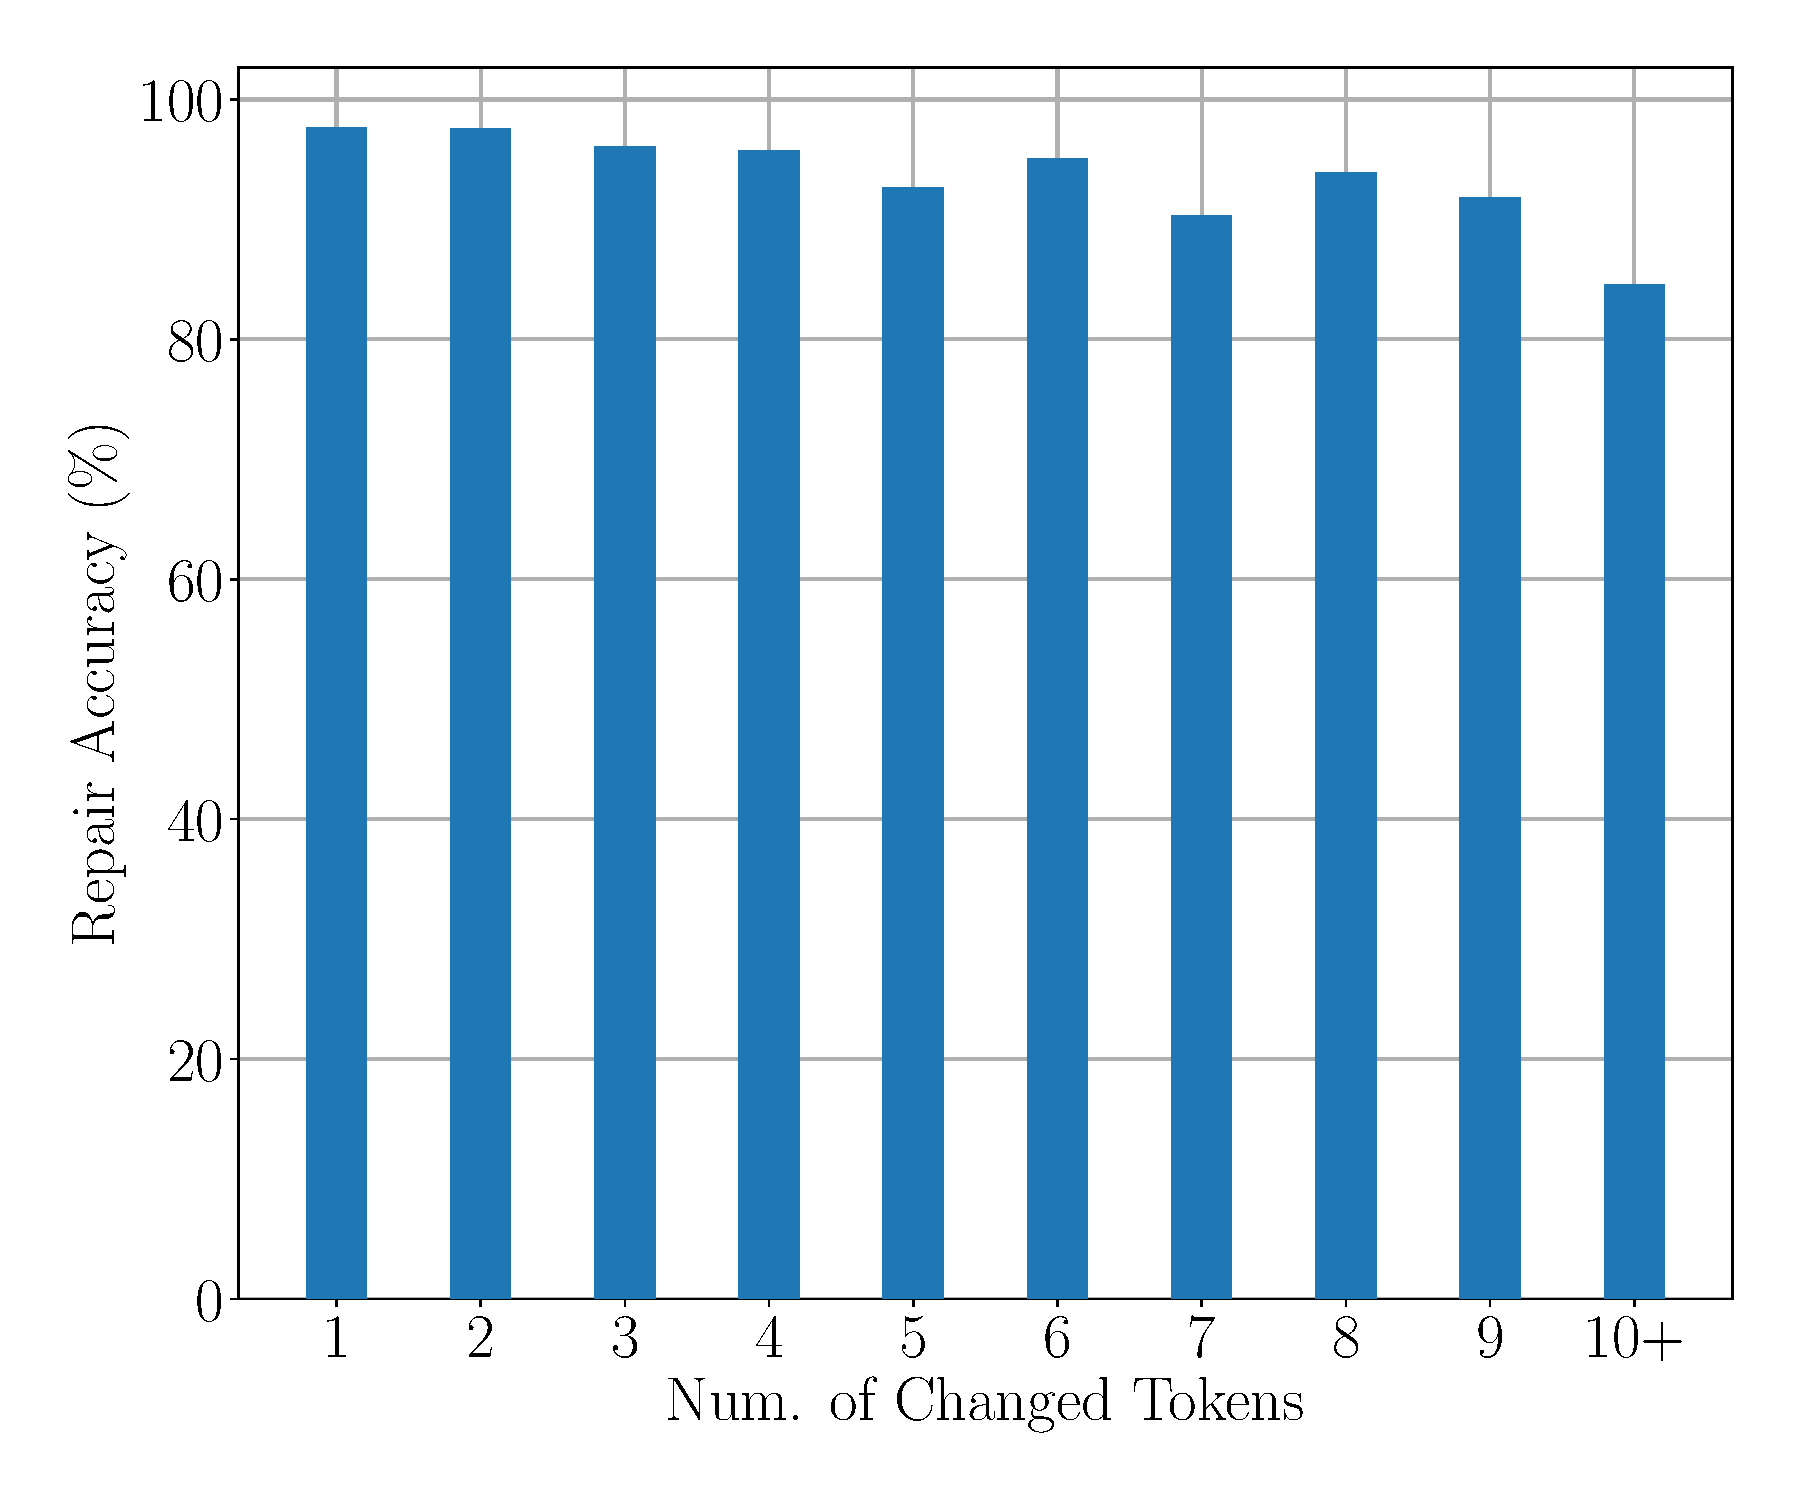
\includegraphics[width=\linewidth]{accuracy-per-change.pdf}
  %   \caption{The repair accuracy for the number of edits needed by the user to repair.}
  %   \label{fig:accuracies-per-changes}
  % \end{minipage}
\end{figure}
